\section{Proposed Methods}


\subsection{Skimming}

\begin{frame}{The Solution: Document Skimming}

\begin{itemize}
  \item This approach is inspired by the fast reading technique "skimming".
  \item<2-> It involves reading while skipping some parts of the text for efficiency.
  \item<3> Reader attempts to skip the redundant or irrelevant parts.
\end{itemize}

\only<1>{
	\vskip 3.4cm
}

\only<2->{
	\vskip .5cm
	\begin{figure}
		\centering
		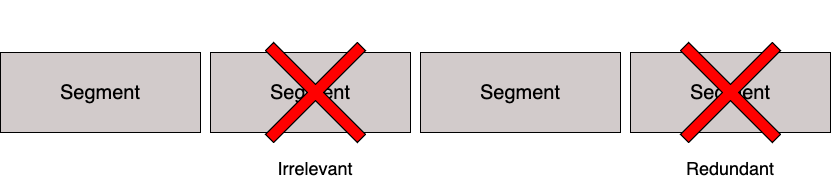
\includegraphics[width=\textwidth]{Images/skim.png}
	\end{figure}
}

\end{frame}

\begin{frame}{Document Skimming (Contd.)}

\begin{itemize}
	\item This method involves uniformly sampling the text segments to fill the LLM's
	context size.
	\item<3-> This ensures we capture details from every part of the text.
	\item<4> A similar approach is taken by \citet{wang2024videoagent} to develop
	VideoAgent for QA on long videos.
\end{itemize}

\only<1>{
	\vskip 3cm
}

\only<2->{
	\vskip 1cm
	\begin{figure}
		\centering
		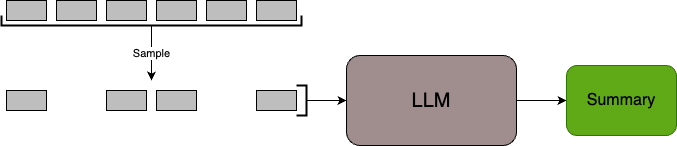
\includegraphics[width=1\textwidth]{Images/doc-skim.png}
	\end{figure}
}

\end{frame}


\subsection{Skimming w/ Extraction}

\begin{frame}{Document Skimming with Extraction}

\begin{itemize}
	\item Instead of randomly sampling the text segments, we can make use of important
	keywords or phrases from the text for sampling.
	\item<2-> This can be achieved by using extractive summarization algorithms that can
	efficiently handle very long texts.
	\item<3-> We can then compute a probability distribution for the segments using
	similarity scores.
	\item<4> We will be experimenting with: TextRank, LexRank, PacSum, Luhn's algorithm,
	and SummaRuNNer.
\end{itemize}

\end{frame}


\subsection{Using Convolutions}

\begin{frame}{Summarizing using Convolutions!}

\begin{itemize}
	\item This approach starts by segmenting the text and encoding the segments.
	\item<2-> Since the segments will be short, we can use a small encoder to efficiently
	encode the them.
	\item<3-> We will then use 1D convolutions as an efficient substitute to the
	quadratic self attention!
	\item<4-> A similar methodolody is applied by \citet{chen2022long} to classify long
	Chinese news.
	\item<5> Longformer \citep{beltagy2020longformer} uses windowed self attention to
	reduce the complexity, but ours is cheaper.
\end{itemize}
	
\end{frame}


\subsection{Central truncation}

\begin{frame}{Back to basics: Truncation}

\begin{itemize}
	\item The most common and straightforward approach used in practice to handle texts
	exceeding the context size is truncation.
	\item Generally, sequences are truncated from the end before processing.
	\item \citet{sun2019fine} find that truncating the middle produced better results
	than truncating the beginning or end.
	\item Their results show that it is even better than more complex hierarchial
	methods!
	\item \citet{worsham-kalita-2018-genre} also find promising results by truncating
	the beginning or the end for summarizing long documents.
\end{itemize}

\end{frame}
